\documentclass[article]{elsarticle}

\usepackage{lineno,hyperref}
\modulolinenumbers[5]

\journal{Computer Physics Communications}

%% `Elsevier LaTeX' style
\bibliographystyle{elsarticle-num}
%%%%%%%%%%%%%%%%%%%%%%%

\begin{document}

\begin{frontmatter}

\title{REST-for-Physics, a ROOT-based framework for event oriented data analysis and combined Monte Carlo response.\\ \includegraphics[height=25mm]{RESTlogoFull.png}}
%\tnotetext[mytitlenote]{Fully documented templates are available in the elsarticle package on \href{http://www.ctan.org/tex-archive/macros/latex/contrib/elsarticle}{CTAN}.}


%% Group authors per affiliation:
\author{Konrad~Altenm\"uller}
\author{Susana~Cebri\'an}
\author{Theopisti~Dafni}
\author{David~D\'iez-Ib\'añez}
\author{Javier~Gal\'an\corref{mycorrespondingauthor}}
\ead{javier.galan@unizar.es}
\author{Javier~Galindo}
\author{Juan~Antonio~Garc\'ia}
\author{Igor~G.~Irastorza}
\author{Gloria~Luz\'on}
\author{Cristina~Margalejo}
\author{Hector~Mirallas}
\author{Luis~Obis}
\author{Oscar~P\'erez}

\address{Center for Astroparticles and High Energy Physics (CAPA), Universidad de Zaragoza, 50009 Zaragoza, Spain}

\author{Ke~Han}
\author{Kaixiang~Ni\corref{mycorrespondingauthor}}
\ead{bur\_ning@sjtu.edu.cn}
\address{INPAC; Shanghai Laboratory for Particle Physics and Cosmology; Key Laboratory for Particle Astrophysics and Cosmology (MOE), School of Physics and Astronomy, Shanghai Jiao Tong University, Shanghai 200240, China}
%\fntext[myfootnote]{Since 1880.}

%\author[irfu]{Damien Neyret}

\author{Yann~Bedfer}
\author{Barbara~Biasuzzi}
\author{Esther~Ferrer-Ribas}
\author{Damien~Neyret}
\author{Thomas~Papaevangelou}
\address{IRFU, CEA, Universit\'e Paris-Saclay, F-91191 Gif-sur-Yvette, France}

\author{Cristian~Cogollos}
\author{Eduardo~Picatoste}
\address{Institut de Ci\`encies del Cosmos, Universitat de Barcelona, Barcelona, Spain}
\address{Departament de F\'isica Qu\`antica i Astrof\'isica, Universitat de Barcelona, Barcelona, Spain}
%% or include affiliations in footnotes:

%\author[irfu]{Yann Bedfer}
%\author[capa]{Susana~Cebri\'an}
%\author[capa]{Theopisti~Dafni}
%\author[capa]{David~D\'iez}
%\author[capa]{Javier~Gal\'an\corref{mycorrespondingauthor}}
%\ead{javier.galan@unizar.es}
%\author[capa]{Juan~Antonio~Garc\'ia}
%\author[sjtu]{Ke~Han}
%\author[capa]{Igor~G.~Irastorza}
%\author[capa]{Gloria~Luz\'on}
%\author[sjtu]{Kaixiang Ni\corref{mycorrespondingauthor}}
%\ead{bur\_ning@sjtu.edu.cn}
%\author[irfu]{Damien Neyret}
%\author[capa]{Luis~Obis}
%\author[capa]{Oscar~P\'erez}



\cortext[mycorrespondingauthor]{Corresponding author}
%\ead{support@elsevier.com}


%%%% INSTITUTIONS %%%%%
%\address[capa]{Center for Astroparticles and High Energy Physics (CAPA), Universidad de Zaragoza, 50009 Zaragoza, Spain}

%\address[sjtu]{INPAC and School of Physics and Astronomy, Shanghai Jiao Tong University, Shanghai Laboratory for Particle Physics and Cosmology, Shanghai 200240, China}

%\address[irfu]{IRFU, CEA, Universit\'e Paris-Saclay, F-91191 Gif-sur-Yvette, France}

%%%%%%%%%%%%%%%%%%%%%%%

\begin{abstract}

 The REST-for-Physics (Rare Event Searches Toolkit for Physics) framework is a ROOT-based solution providing the means to process and analyze experimental or Monte Carlo event data. Special care has been taken on the traceability of the code and the validation of the results produced within the framework, together with the connectivity between code and data stored registered through specific version metadata members.



The framework development was originally motivated to cover the needs at Rare Event Searches experiments (experiments looking for phenomena having extremely low occurrence probability like dark matter or neutrino interactions or rare nuclear decays), and its components naturally implement tools to address the challenges in these kinds of experiments; the integration of a detector physics response, the implementation of signal processing routines, or topological algorithms for physical event identification are some examples. Despite this specialization, the framework was conceived thinking in scalability, and other event-oriented applications could benefit from the data processing routines and/or metadata description implemented in REST, being the generic framework tools completely decoupled from dedicated libraries.

REST-for-Physics is a consolidated piece of software already serving the needs of different physics experiments - using  gaseous Time Projection Chambers (TPCs) as detection technology - for background data analysis and detector characterization, as well as generic detector R\&D. Even though REST has been exploited mainly with gaseous TPCs, the code could be easily applied or adapted to other detection technologies. We present in this work an overview of REST-for-Physics, providing a broad perspective to the infrastructure and organization of the project as a whole. The framework and its different components will be described in the text.

% Detector physics

\end{abstract}

\begin{keyword}
Software architectures (event data models, frameworks and databases)\sep Simulation methods and programs\sep Data processing methods\sep Rare Event Physics Searches\sep neutrino \sep axion \sep dark matter
\end{keyword}

\end{frontmatter}

\linenumbers

\section{Introduction}
\label{sec:intro}

% What it is?
REST-for-Physics (Rare Event Searches Toolkit for Physics) is a collaborative software effort providing a common framework and tools for acquisition, simulation, generic data analysis, and detector response in experimental particle physics. An ambitious feature of REST-for-Physics is its capability to analyze together and compare Monte Carlo and experimental data using the same \emph{event processing} routines upon a unified \emph{event data} - \emph{metadata} architecture. 

% Describe motivation. 
The framework was born to bring together different software requirements related to gaseous Time Projection Chambers (TPCs) in the context of Rare Event Searches, and to unify and coordinate various independent developments in a common, modular infrastructure with potential for scalability and reusability. Special care has been taken to ensure the traceability and reproducibility of the results obtained after the data processing, linking the code version with the metadata version stored on disk, and protecting such relation. Any user local changes to the code are identified at compilation time. This is used to guarantee that the version executed and the results written to disk correspond to an unmodified official public release. This fact is extremely relevant when planning to register official experimental data and preserve it for historical reasons, such as covering the data management plan of scientific collaborations, including the release  of data to be publicly exploited outside the collaboration domain. The code updates are periodically published at the Zenodo citations system, where one finds the latest official release today\,\cite{javier_galan_2021_5092550}.

% Add historical context
REST-for-Physics is the result of several years of experience on detector physics and research, motivated originally to cover the software needs of the T-REX project for neutrino and dark matter searches~\cite{Irastorza:2015dcb,Irastorza:2015geo}. The REST-for-Physics code has benefited from several academic works, as it becomes apparent in several PhD thesis publications\,\cite{IguazThesis,tomas2013development,SeguiThesis,HerreraThesis,GraciaThesis, GarciaPascualThesis, RuizThesis} that have contributed to shape and define the final project that we describe in this manuscript.
This project has contributed to the development of different but interconnected research activities in a coherent way, unifying common tools that are used today regularly not only in research but also at all the academic levels, from undergraduate to master students. 

% REST-in-a-nutshell

% Research and experiments, distribution.
Different experimental projects have seen REST-for-Physics growing from its preliminary stages to the mature project we present in this work. REST-for-Physics has been evolving within, and it is being used to produce results at, CAST~\cite{Anastassopoulos:2017ftl}, TREX-DM~\cite{trexdm_bckmodel}, PandaX-III~\cite{pandaxiii_cdr,Lin:2018mpd,Galan:2019ake}, and IAXO~\cite{Armengaud:2019uso}. Those projects have benefited from the consolidation of REST as a common tool widely used among collaborators to process, register and analyze detector data. We foster the use and development of REST in other experiments in a community effort to maintain appropriate tools for related tasks. In addition to sharing the know-how and experience in our physics domain, the motivation to release a public common framework resides in providing the possibility to distribute the experimental data following a unique format readable with REST-for-Physics, or any other ROOT I/O compatible code in a future open-data program of the experiments. The code is open-source and it is distributed under a GNU public license at \emph{GitHub}\,\cite{REST_Git}.

% Introducing scope of this paper
The aim of this document is to give the reader a broad perspective of the purpose of the software project, its organization and contents, and the basic instruments that shape the whole infrastructure, giving an idea of its scalability potential, and in addition, showing the code validation strategy and continuous integration philosophy. For further reference we refer to detailed information, including an API class documentation for developers\,\cite{REST_API}  synchronized daily with the latest development version, and a comprehensive guide for first time users\,\cite{REST_user_guide}. We also offer an additional communication channel in the form of a public forum\,\cite{REST_forum} to encourage discussion about topics related in our domain, help others on their first steps using REST and/or integrate their first routines inside the framework, and discuss about new or existing feature upgrades.
\section{REST conceptual design and scope}
\label{sec:conception}

REST-for-Physics defines common data structures for event-based data processing. As we will see later on the general description (at section\,\ref{sec:framework}) this entails a prototyping of the event data holder, the processes that transform or operate those data holders, and the description of the metadata information giving a meaning to the data being processed; such as initial data taking conditions, input processing parameters, or output results written to disk in the form of metadata.
The prototypes to event data, processes and metadata are complemented  with basic analysis tools that are frequently used on event-based data analysis. Another important structure, named tree, is used to gather relevant event information during the data processing. This analysis summary tree contains a set of variables defined during the event data processing to be used in subsequent higher level analysis.

The intention of REST-for-Physics is to define a framework, or code development space, that centralizes related event processing and analysis routines, being those routines contributed by the same experts that work on the analysis of the data. The REST community keeps a strong link between the algorithm design and the framework design, since there is an implicit connection between the algorithm development, analysis interpretation, and framework design requirements. REST provides already existing processes that we will be able to use directly to define a given event processing task. Anyhow, REST has been designed to provide the means to be extended with new processes, metadata or event data types.

The development of REST emerges in a strong academical environment. In such context, REST intents to provide the means for academic works to materialize in the form of a piece of code that can be re-used within an already consolidated software infrastructure. A major goal for REST is to make it more accessible to non-computing experts that have a high level for algorithm coding abstraction and comprehension of the physics context.

REST-for-Physics does not replace or compete with other dedicated simulation packages which provide high accuracy physics description on dedicated problems, but it seeks to integrate those packages, such as Geant4~\cite{Agostinelli:2002hh} or Garfield++~\cite{Garfield}, and exploit them inside the framework as needed on the processing of the event data. In addition, REST-for-Physics includes dedicated libraries (described at section\,\ref{sec:libraries}) that implement specialized algorithms for signal processing or physical track reconstruction. We develop our own algorithms for known mathematical problems, e.g. time signal processing, to have full control over those  and adapt them to our experimental needs, while still linking to consolidated libraries when possible, as it is for example the case for high-precision numbers implementation at the \emph{mpfr} library\,\cite{10.1145/1236463.1236468} or the use of graph theory methods\,\cite{Applegate:2007:TSP:1374811,concorde}.
\section{General description}
\label{sec:framework}

% Table with useful information, code version, github address, zenodo reference, documentation

% Mention physics units, basic geometrical routines TRestPhysics, TRestMesh, ...

REST-for-Physics is composed of a set of libraries written in C++ and it is fully integrated with ROOT~\cite{ROOT,Brun:2011Gp,ROOT2011}, i.e. most C++ classes inherit from a ROOT TObject and therefore they can be read, accessed or written using the ROOT I/O interface. The only structural dependence is related to ROOT libraries, while other packages, as \emph{Geant4}~\cite{Agostinelli:2002hh} or \emph{Garfield++}~\cite{Garfield}, can be optionally integrated and used within the REST-for-Physics framework when generating or processing Monte Carlo data. Being REST-for-Physics a natural extension of ROOT, we follow the same naming conventions, which are the Taligent rules. On top of those standard naming conventions, any REST-for-Physics C++ class (object) will be always started by the \emph{TRest} prefix. In this manuscript we will highlight the words when they clearly make a reference to an existing REST-for-Physics C++ object. I.e. an object named \emph{TRestEvent} will be written in the following as \emph{event} or an object named \emph{TRestAnalysisTree} will be written as \emph{analysis tree}. Therefore, a highlighted word, within context, expresses a deep connection with the different elements of the code.

%%%%%% THE MAIN FRAMEWORK DESCRIPTION %%%%%%%
\subsection{The REST-for-Physics framework}
Inside the REST-for-Physics ecosystem we may distinguish a main library, or framework, that prototypes and fixes the implementation of most of the REST-for-Physics elements. Those base objects serve to define common methods and data members for specific\footnote{The reader should notice that when we refer to specific objects, we refer to objects which inherit, in the strict sense of C++ object inheritance, from the base abstract objects, \emph{event}, \emph{metadata} and \emph{event process}. In the text, we will highlight the keyword \emph{specific} to refer to those inherited objects in a generic way, i.e. \emph{specific event} will be connected to any \emph{TRestSpecificEvent} or \emph{specific event process} would be connected to any \emph{TRestSpecificProcess}. It is worth to notice that event and process objects contain the \emph{event} and \emph{process} keywords in their class name, while metadata classes usually omit the use of the \emph{metadata} keyword. } objects. We shall briefly introduce those basic elements.

\begin{itemize}
    \item The \emph{event} object encapsulates any specific \emph{event} data inside REST. It defines common fields, such as timestamp or event id, and it prototypes common methods used for printing or drawing event information. A particular \emph{specific event} implementation defines a type, thus in what follows we will distinguish between the \emph{event} data as the explicit contents of a particular \emph{specific event}, and the \emph{event} type as the format, or structure, of the \emph{specific event}.
    
    \item A \emph{metadata} object can be initialized through a configuration file (at present we adopted the XML format). A \emph{metadata} class might be used as a mere information container, storing relevant parameters, that can be initialized through XML, such as the conditions of a \emph{Geant4} simulation, i.e. the \emph{geant4} metadata object, or it might adopt the shape of a complex object definition that implements advanced methods, such as the implementation of a \emph{detector readout}, or a \emph{magnetic field} volume including interpolation routines. Those advanced \emph{metadata} objects will be found at specialized libraries, some of them being detailed later on in section\,\ref{sec:libraries}. Conceptually we understand by \emph{metadata} any information required to give meaning to any \emph{specific event} data. Therefore, any input or output parameters, required during the processing or transformation of \emph{event} data, or type, using \emph{event processes}, is regarded also as \emph{metadata}. 
    
    \item The \emph{event process} object defines an input/output \emph{event} scheme allowing to interconnect different \emph{specific event process} implementations into a sequential processing chain. The \emph{event process} inherits itself from the \emph{metadata} object, since a process usually requires initialization to define few input parameters that control the behaviour of the process.
\end{itemize}

We will find other basic or elemental tools inside the main framework, such as output string helper methods, fundamental physics constants and units system, or other basic mathematical tools helping to the development of any specific \emph{event process}. Any \emph{metadata} or \emph{event process} object that does not require specific specialization will be likely hosted inside the framework domain.
 On top of that, the framework repository\,\cite{REST_Framework_Git} serves to centralize other REST-for-Physics components, such as libraries or packages. Those components will be introduced later in section\,\ref{sec:libraries}.%SUB-MODULES

% Describe sub-modules, libraries and packages.

% framework core, tools, analysis

% define \emph{metadata} to TRestMetadata naming convention

% Submodules, Libraries, packages, projects

%%%%%% I/O Access and storage %%%%%%%
\subsection{I/O access and metadata storage}

%% Paragraph dedicated to REST progress and philosophy % Description of metadata+data concept
%% During the last years, major upgrades took place on the REST core libraries\,\cite{Galan_8thTPC}. 


% TRestRun (any event data processing taking place with REST will write to disk a TRestRun object, any REST object taking active part on the data processing will be stored in ROOT file.
REST-for-Physics uses the ROOT I/O interface to write \emph{event} and \emph{metadata} objects to disk. A ROOT file generated with REST may contain any number of \emph{specific event} and \emph{specific metadata} objects, including any \emph{specific event process} (being a \emph{metadata} object itself). Those objects are stored in a unique file, together with the \emph{run} metadata object and the \emph{analysis tree} that are always present at any file that has been processed with REST. The \emph{run} object registers few important values to identify the data file, such as the start time, duration, run number, etc, while the \emph{analysis tree} collects information, named observables, at any stage of the data processing. The \emph{run} object takes also an active role when accessing the different objects stored on disk by implementing helper methods to access the data, such as getting a list of events fulfilling particular conditions at the \emph{analysis tree} or retrieving directly the pointer to a given event id number, and updating simultaneously its corresponding \emph{analysis tree} entry.

% something about metadata
% For each aspect of \emph{metadata}, we define a class with proper data members to describe it, known as \emph{metadata} structures. 
The framework philosophy is to create \emph{specific metadata} objects with dedicated data members to store any information crucial for the final analysis, and/or to fully determine the nature of the data we are storing. All the \emph{metadata} inherited objects gain data member reflection support, thus creating a relation between the C++ conceptual class members and the text fields used in our configuration files. Through the implementation of the \emph{metadata} object we have designed a dedicated file format for REST, based on Extensible Markup Language (XML). This upgrade allows us to read XML files with additional features, such as using system environment variables, complex programming instructions, including \emph{if} conditions or \emph{loops}, evaluation of mathematical expressions, or support for arbitrary physical units conversion inside any parameter. We assign a new extension \emph{rml} to this upgraded XML format.

Using the \emph{metadata} philosophy we create a unique relation between the configuration files and the C++ objects. One XML element is identified with one \emph{metadata} object, with its attributes associated to the data members inside the object. If there is an embedded element inside the XML element, it is associated in-chain to the corresponding \emph{metadata} member of the element. In this way, the automatic initialization of \emph{metadata} objects is achieved, without any file reading methods in the class.

%% RML --> system environment variables + loops + mathematical expression evaluation + physical units support in parameters



%% SHALL WE ILUSTRATE THIS WITH SOME CODE? Such as Int\_t fMetadataMember = 0;   is connected with `<parameter name="metadataMember" value="10"/>? 


% A link is therefore established between class data members and text fields, enabling automatic reading of configuration files. We invented a file format for REST, \emph{rml}, based on Extensible Markup Language(xml). We believe the strong hierarchy and attribute sets provided by xml are beneficial in our application. All the running jobs, such as simulation, analysis, and file generation, are based on \emph{rml} encoded configuration file. 

%% metadatda and rml. Shall we explain rml?
% rml --> metadata class's data members. We now set a convention for rml parameters linked to metadata class's data members. **configurability** could be explained on "reflectable metadata"


%%%% This paragraph will be considered at detector library, and at data processing chain.
%% In addition to the storage of value sets, we have various tool methods provided by the \emph{metadata} structures which is useful in the analysis. For example in detector readout topology we enable readout channel position finding according to the daq ID, and in gas property we can calculate electron drift speed with certain external libraries.Any created \emph{metadata} structures will be stored to the output file. Moreover, any previous existing \emph{metadata} structures from input file will be transferred to output file. Traceability and reproducibility of REST data would be enhanced with this file logic. 

% something about event data
%% Basic introduction of data types and processes
% An event type defines a particular structure that helps organizing different entities that keep a similar relation.
%%% Multiple event types(data structures) are also defined in REST to store \emph{event data}, which could be generated either in data acquisition, simulation or data processing. The inherited common data fields, such as event id, time, tag, keeps continuity of data flow, while the special fields contained in each types conduct best structured data for different stages of analysis. Common interfaces are also implemented for visualizing and printing the \emph{event data} for each type of event. In addition, we also implemented various tool methods associated to the nature of each data structure, for example points rotation, Fast Fourier Transform (FFT), which helps to develop analysis code quickly. Each type of \emph{event data} is stored in an individual branch in the tree in the output file, helping to check the condition of each stage of analysis.

\subsection{Event data processing and analysis}

The framework allows us to build an event data processing chain in a modular way by interconnecting already existing \emph{specific event processes}, or to develop new ones with the potential to plug it directly to an existing processing chain. Each \emph{event process} has access to the input \emph{specific event}, the \emph{analysis tree} (described later in this section), and any \emph{metadata} object that it is accessible by the \emph{run} object. Depending on the input/output \emph{specific event} interaction inside the process we may attempt to classify the \emph{event processes} into different groups, as illustrated on Figure\,\ref{fig:dataChain}.


%%% It seems we have a bit of confusion on this topics. Hope the new version is more clear 

\begin{itemize}
\item An \emph{external process} is a process that reads an external data source, usually at the beginning of a REST processing chain. It might be binary data generated by an acquisition system, or Monte Carlo data generated by an external simulation package. The process will be in charge of understanding the format of that external data serving to initialize a REST \emph{specific event}.

\item An \emph{internal transformation process} is a process in which the \emph{specific event} input is the same type as the \emph{specific event} output. The \emph{event} data will be transformed but not the \emph{event} type.

\item A \emph{pure analysis process} accesses the information of a \emph{specific event} type and produces observables that will be added to the \emph{analysis tree} but it will not modify the \emph{specific event} in any sense. A pure analysis process might serve, for example, to implement a complex physics model that uses the \emph{specific metadata} and \emph{specific event} information to elaborate some results that will be exported to the \emph{analysis tree}, or a \emph{specific metadata} object.

\item A \emph{general process} is a process that does not access the information inside the \emph{specific event} type. It will only need access to the basic \emph{event} information common to all \emph{specific events}, or the \emph{analysis tree}. Therefore, this process may be plugged at any point of a data processing chain without restrictions. Processes of this kind might have many different purposes as it could be; to visualize online data on real time, implement a \emph{summary} process to calculate averages (or any other statistical variable) from the \emph{analysis tree}, or perform a generic fitting of a variable at the \emph{analysis tree} spectra placing the fitting results at a dedicated metadata object, between many other basic analysis tasks.

\item A \emph{transformation process} is a process that receives as input a \emph{specific event} and transforms it to a different \emph{event} type. This kind of processes will be all placed at the \emph{connectors} library, described on section\,\ref{sec:libraries}, in order to encapsulate all library inter-dependencies at a single entity. 
\end{itemize}

%% This figure is available here: https://docs.google.com/presentation/d/1a2gdqvANFdbIq_GCrF9XQyBjAOBtZc5N9xahquPdVpE/edit?usp=sharing
\begin{figure}[h]
  \centering
  \raisebox{-0.5\height}{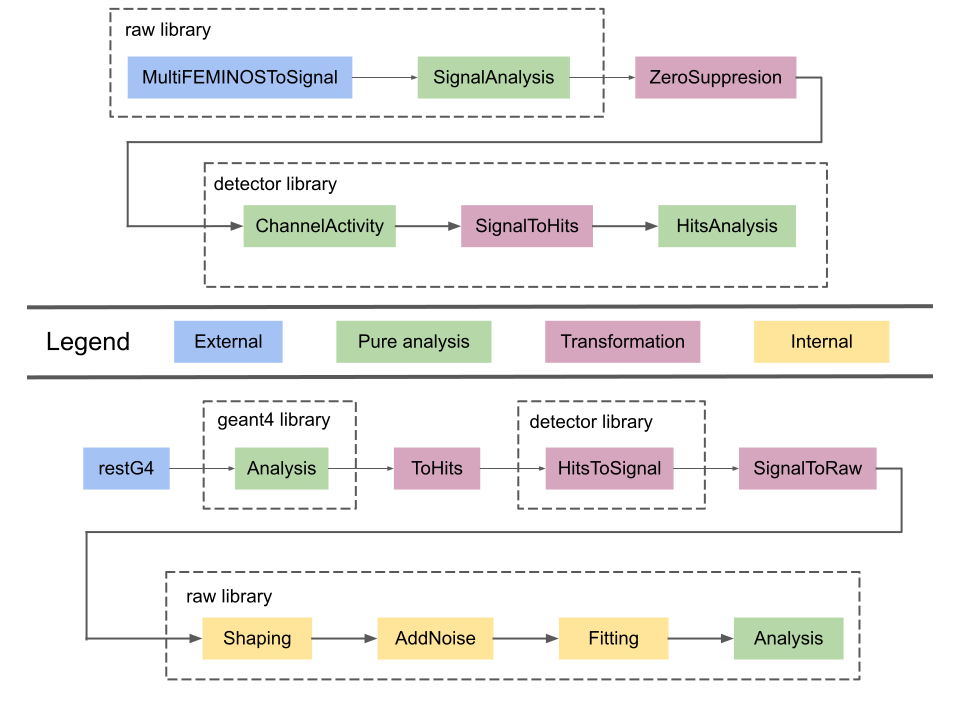
\includegraphics[width=0.95\linewidth]{images/DataChain.pdf}}
	\caption{An schema showing the event data flow for two different data chain implementations in order to illustrate the different processes classification. On the \emph{top}, an experimental detector data processing chain reading a binary file, analysing, and post-processing the rawdata for event reconstruction. On the \emph{bottom}, a Monte Carlo generated data processing chain, where the data is analysed and transformed to match the data format in a raw electronics acquisition system, where we condition the data using \emph{shapping}, \emph{add noise} and \emph{fitting} internal processes belonging to the raw library. We observe in this schema how different libraries (described later on section\,\ref{sec:libraries}) intervene at different stages, and how those play a role on both, Monte Carlo and experimental data.}  \label{fig:dataChain}
\end{figure}

% Event transformation
A \emph{specific event} might be transformed during the event processing and, in that transformation, relevant information might not be available anymore at the final transformed output event. The reason is that the role of the \emph{specific event} object is to provide a faithful or significant representation of the data at the state of processing where we are inside our processing chain, i.e. at different processing stages we might have the event data made of time signals registered at an electronics setup, or we might have the event data in the shape of discrete energy deposits at a physical coordinate system. Therefore, the transformation from one event data representation, or \emph{specific event}, into another, carries as a consequence that a relevant parameter available at a particular stage, is not available anymore (or it is harder, less intuitive, accessing to it). 

% Analysis tree description
The \emph{analysis tree} comes into play as an instrument to collect all those parameters extracted or calculated from the \emph{specific event} information and that will be relevant for the final analysis.  Any \emph{specific event process} in the processing chain is allowed to add new observables to the \emph{analysis tree}. Once a process adds an observable to the \emph{analysis tree} this observable will be always available even if the \emph{event} data is transformed or the processing chain happens in several steps using different input/output REST data files. The information at the \emph{analysis tree} is always accumulative, and therefore it will contain a full summary of the observables added by each process (see Figure\,\ref{fig:observables}).
%, following the decisions taken by the person in charge of the data chain design. 
In brief, the \emph{analysis tree} provides a way for \emph{specific event processes} to export an analysis result, extracted from each event, to the framework. It must be noticed that processes have two ways to export results, an event per event based observable inside the \emph{analysis tree}, or a given result common to all the events in a particular \emph{run}, that will exported in the form of a \emph{specific metadata} object.

\begin{figure}[h]
  \centering
  \raisebox{-0.5\height}{
  \begin{tabular}{c}
  \includegraphics[width=0.98\linewidth,trim=0 0 10 0, clip]{images/TBrowser.png} \\
  
  \\
  
  \includegraphics[width=0.65\linewidth,trim=0 98 0 0, clip]{images/observables.png} \\
  \end{tabular}
  }
	\caption{Two computer snapshots showing the observables registered at the analysis tree. On the \emph{top}, inspecting the observables using a ROOT TBrowser object. On the \emph{bottom}, inspecting the analysis observable values registered at a particular event entry using the ROOT command line interface.}\label{fig:observables}
\end{figure}


The information extracted by a process and added to the \emph{analysis tree} might be as simple as just a registered value available at the \emph{specific event} at a given stage of the processing chain, or it might be the result of a complex calculation in the context of a physics model, including complicated input \emph{metadata} objects or parameters. Of course, even in the case of basic observables extracted directly from the \emph{specific event}, the user might be interested to know the evolution of such observable after an intermediate processing. In order to do that, it is possible to define the same \emph{specific event process} twice at different positions in the sequential processing chain.


%defines a particular analysis job upon a particular input event in order to manipulate the \emph{specific event} data, transform it and extract relevant information. 

%Afterwards the \emph{event process} must yield an output event. 

%In principle, any \emph{event process} that participates in a data processing chain must satisfy that its input event type corresponds with the output event type of the previous \emph{event process}. 

The \emph{event process} object implements a method to facilitate the addition of observables to the \emph{analysis tree}. This method allows to create automatically a new observable from any C++ variable (including various C++ types, from base types to proper \emph{stl} containers). We do not need to care about global values and their addresses by using this method. Weakening the concept of a ROOT \emph{branch} and \emph{tree} helps us to reduce the number of lines in the code, while focusing more on analysis.

%% discuss how to analyze Monte Carlo and experimental data using common event processes
Our framework design is completely transparent to the processing of real experimental data, or Monte Carlo simulated data. The reason is that a \emph{specific event process} implementation may operate on both scenarios. The only requirement is that the experimental or simulated input \emph{event} must be given to the process in the form of a \emph{specific event} type. If both, simulation or experimental data, are conditioned to fit in a common \emph{specific event} type, we will be able to build a processing chain that not only processes simulated data or experimental data, but that fully combines both. As a hypothetical case, we could integrate a process simulating the signal shaping of electronics into real experimental data to assess the benefit of applying such electronics setup in our real experiment. Furthermore, a proper conditioning of the generated Monte Carlo \emph{event} data will allow us to evaluate the algorithms for analysis to be used with the real experimental data even before the start of the physics data taking program.

%Either Monte Carlo or experimental data can be the input of \emph{event processes}. 
% For the Monte Carlo data, with properly conditioned simulation \emph{event processes}, we can reproduce the raw data of the detector acquisition. Once at that stage, by reusing common \emph{event processes}, we can analyze the simulation data just as experimental data. Algorithms can be developed with optimized data selection efficiency even before 


% Discuss the analysis tree(what's better than basic tree) and idea of observable
%REST provides an uniformed target, \emph{observable}, for the \emph{event processes} to export analysis result. 
%\emph{Observable} is defined as any information extracted from \emph{event data}. 
%It could be the raise times of each pulses in an event, the reconstructed event vertex/energy, the background likelihood of the event, etc. 
%Multiple \emph{observables} can be associated to the \emph{event data}, forming a list of event properties. 


%% discussion about multi thread 
Event processes are executed through an efficient engine with multi-thread support. The data processing chain is cloned into multiple instances and kept in different threads respectively. During execution, the input event is in turn dispatched to each thread for processing, while the output event is redirected to the global output file for writing, leading to an increase of processing speed proportional to the number of threads enabled. Figure\,\ref{fig:processing} summarizes the input/output processing logic and the different concepts previously described in this section.   %Multi-thread operation is most helpful in case of algorithm verification, for example we can quickly get the result of a newly added observable to see if the code is alright.

\begin{figure}[htb!]
  \centering
  \raisebox{-0.5\height}{
\includegraphics[width=0.75\linewidth]{images/process_chain.png}}
	\caption{A schematic showing the event data flow inside a REST processing chain. The \emph{run} object is initialized, and it has access to any \emph{specific metadata} or \emph{event} data available at the input REST file, or any additional objects described through \emph{rml}. The data is then processed using the implementation inside the \emph{process runner} object. Different event types (A,B,C,D) make reference to different \emph{specific event} implementations. The resulting output REST file will contain all the \emph{metadata} information available to the chain, including any previously available, together with the transformed output \emph{specific event}, and the updated \emph{analysis tree}.  }\label{fig:processing}
\end{figure}


% Define different event processing types: pure analysis.

% - Specific analysis process. It needs to access a particular event data type (it will be placed then at the corresponding library defining that event type).
% - Pure analysis process. It only requires access to the analysis tree (and therefore it will be placed at the main framework).
% - Conversion process. It is a process that interconnects 2 libraries by transferring an event type into another. Therefore, this kind of process will be placed at the dedicated `connectors` library.
% We usually write \emph{event processes} in two major ways, identified by whether transforming the type of \emph{event data}. If the output event is transformed into another type, it is a \emph{conversion process}. If it operates in a particular event type, i.e. \emph{hit}, \emph{raw signal} or \emph{track processes}, in which the output event type remains unchanged, it is an \emph{analysis process}. In the following sub-sections we provide a description of the different processes involved in our data processing. A full, detailed and up-to-date list of documented processes will be available at~\cite{RESTsultan} for further reference.

\subsection{Visualization and plotting}

% TRestBrowser --> event by event **visualization**
% TRestAnalysisPlot --> data statistics plot, histo
% TRestMetadataPlot --> for metadata

REST-for-Physics implements routines for event visualization and observable plotting based on ROOT drawing objects and methods. We use ROOT graphical interface objects to create basic tools, such as an \emph{event browser} with a control panel and a drawing pad (see Figure\,\ref{fig:eventBrowser}). The drawing pad itself is the target of the \emph{draw event} method implemented at each \emph{specific event}. If enabled, different output \emph{specific event} trees - from different stages at the data processing - will have been stored in the same file. In that case the \emph{event browser} will be able to switch between the different event data representations.

\begin{figure}[h]
  \centering
  \raisebox{-0.5\height}{\includegraphics[width=0.45\linewidth]{images/EventBrowser.png}\,\,\,\,\includegraphics[width=0.45\linewidth]{images/EventBrowserSelection.png}}
	\caption{Two snapshots from the REST \emph{event browser} where we observe the control panel and the drawing pad showing an event entry for a \emph{raw signal event} (see section\,\ref{sec:libraries} for details on the \emph{specific event} type). On the left figure we present the complete event, while on the right figure the pulses have been filtered using an option passed to \emph{draw event} method implemented at each \emph{specific event}.}\label{fig:eventBrowser}
\end{figure}

%%%%%%%%%%%%%%%%%%%%%%%%%%%%%%%%%%%%%%%%%%%%%%%%%%%%%%%%%%%%%%%%%%%%%%%
%% This is true, we have the choice to put all them together. But it would be good to implement a kind of "smart" event browser that would open all the previous files used on the processing and contain event data. Then we would create a new TAB for each type on the window PAD, there where it says "TAB 1", "TAB 2".
%%%%%%%%%%%%%%%%%%%%%%%%%%%%%%%%%%%%%%%%%%%%%%%%%%%%%%%%%%%%%%%%%%%%%%%
%% THIS IS AN OPTION
%As described above, multiple event branches are stored in REST output file corresponding to the different stages of data processing. Each type of \emph{event data} contains a default visualization method to be drawn on the pad. When opening the file for visualization, one can simply switch between the entries, and view the \emph{event data} at different stages.
%%%%%%%%%%%%%%%%%%%%%%%%%%%%%%%%%%%%%%%%%%%%%%%%%%%%%%%%%%%%%%%%%%%%%%%

The \emph{analysis tree} object inherits directly from a ROOT TTree object, and therefore we may exploit all the resources provided by ROOT when analysing the observables that have been added to the \emph{analysis tree} by the different \emph{specific event processes} at the processing chain. I.e. we can use a ROOT TBrowser to explore the REST data files, and quickly draw and inspect few variables from the \emph{analysis tree}. 

Furthermore, REST implements dedicated tools for automatic and systematic plot generation, such as the \emph{analysis plot} or the \emph{metadata plot} objects. 
The \emph{analysis plot} will efficiently integrate the capability to merge thousands of files through a \emph{rml} file where we will define the plots that we want to produce with the combined data, including few advanced features such as classifying the produced histograms as a function of any \emph{specific metadata} member stored in the files, or define cuts based on the \emph{analysis tree} observables that serve to filter the data to be plotted. The \emph{analysis plot} object allows us to create a plot definition that can be used, for example, to produce quick analysis reports in \emph{pdf} format or to export histogram data in any other file format supported by ROOT.
The \emph{metadata plot} object will allow us to read many REST generated files and draw any \emph{specific metadata} member as a function of another \emph{specific metadata} member extracted from each of the REST files provided. This will allow us to study for a long data-set the correlation between any two metadata parameters, or to plot the evolution of a metadata parameter as a function of the \emph{run} start time, or the associated run number, for example.

%Histograms of \emph{observables} are generated with REST's analysis plot logic. Pads, plots, axis, legends, or even sub-pads and sub-plots, can all be defined through our \emph{rml} configuration file, ensuring better hierarchy and readability than C++ codes. Multiple files can be merged to a single figure or be classified into different figures. Figures can be drawn into pdf files with a single command. 

% TRestAnalysisPlot, TRestMetadataPlot, ...

\subsection{Execution and job management}
% restRoot, macros, practical data chain processing definition
Two executables are provided on the top level of the REST-for-Physics framework and are always available to any REST user, \emph{restRoot} and \emph{restManager}. 
\emph{restRoot} provides a ROOT interactive prompt with REST libraries loaded, and optionally, with all the available REST macros preloaded. 
\emph{restManager} manages the execution of jobs. It might launch a processing chain defined through the \emph{process runner}, execute a method defined at any REST object available to the \emph{run} object, or launch a ROOT C++ macro file. On top of that, macros might have been assigned an alias to allow the system to launch macros execution through \emph{restManager} with a single command. Packages, or applications, that link to REST libraries will also provide their own executables, such as \emph{restG4} or \emph{restFileIndexer}  (see Figure~\ref{fig:executables}). \emph{restManager} allows to define all those actions through a configurable \emph{rml} file, but on top of that, the \emph{manager}, executed through the \emph{restManager} executable, guarantees that the event data processing flow follows the standards previously described in Figure~\ref{fig:processing}.

\begin{figure}[h]
  \centering
  \raisebox{-0.5\height}{\includegraphics[width=0.9\linewidth]{images/executables.png}}
	\caption{REST executables running logic. \emph{restManager} and \emph{restRoot} work together to provide full access to the REST framework functionalities. Pre-defined ROOT C++ macro files are accessible through different interfaces, as it is shown through the \emph{REST\_ViewEvents.C} macro. Applications based on REST framework (green bubbles) extend the scope of the framework by providing additional functionalities, such as \emph{restG4} or \emph{restFileIndexer}.}
	\label{fig:executables}
\end{figure}

On top of that, a bash script, \emph{rest-config}, is generated at each project compilation to provide information on the configuration of a particular build and to facilitate the linking of REST with external applications. 

\subsection{Project structure, versioning and code validation}
% submodule strategy

The main framework defines the basic functions, and describes the behavior of the main elements of REST. As previously mentioned, it also serves to centralize all the REST-for-Physics components, such as packages or libraries, and eventually dedicated projects. We have adopted a \emph{git submodule}\footnote{From this point we introduce few concepts connected with the code versioning system, \emph{git}, that are broadly available online, such as \emph{commit} or \emph{submodule}. When we refer to those alien concepts we will highlight it using the \emph{git} keyword followed by the specific concept name.} strategy to integrate those components in a modular way inside the main framework repository. This scheme allows us to independently monitor the development activity at each of those components, to isolate technical issues, and to focus on their functionality. Each component evolves independently with its own version or tracking system. A particular state of the code at each of those components is fixed at the main framework through a \emph{git commit} hash, or unique number. When that happens we say that the corresponding \emph{git commit} becomes the official component version of REST.

The framework repository fully centralizes the versioning system of REST, understood as the state of the code at a given period of time, including the state of the official \emph{submodules} attached to it. Any REST \emph{metadata} object written to disk using the ROOT I/O scheme will be stamped with metadata values that assure that the data written to disk has been processed with a given version, or state of the code. In order to certify that, two of those metadata members will be initialized at the code compilation time. The first metadata member will assure the source code was built from a clean unmodified state respect to the \emph{git remote} repository, and the second metadata member will certify that the corresponding framework code state is associated with an official \emph{git tag} release, where each \emph{git tag} generated at the main framework repository will automatically produce a code release referenced and citable at the \emph{Zenodo} system\,\cite{javier_galan_2021_4692983}.

On top of that versioning strategy, it is important to mention that REST properly implements the ROOT schema evolution and assures backwards compatibility for objects that have suffered changes on their data members.

%Those libraries and packages are kept as \emph{git submodules} of REST main framework, with their versions evolving independently. Therefore, the development of \emph{sub-modules} could be separated from the main framework, contributing to a series of git repositories under multi-person work. During installation, specific libraries for different workloads can be selected to download, compile and install.

% no need to explain TRestTask since it doesn't bring new concept

% \subsection{Basic tools}
% versioning strategy
% pipeline  validation

To ensure the code quality and stability with time, each repository integrates a validation pipeline where basic tests on the code are performed, such as code formatting and style validation, testing the proper libraries integration and building of executable programs or, even more important, testing basic results from complex data processing chains (see Figure\,\ref{fig:pipelines}). Each modification to the code, or \emph{commit}, will be verified by running those validation pipelines. If a modification to the code produces an unexpected value on a consolidated data processing routine, the contributor will be notified, and changes will only become official after peer review of the code. This fact is extremely relevant to guarantee that our algorithms keep producing the expected results, or in the undesired case of a bug code identification, promptly identify the affected routines after bug correction. On top of that, validation pipelines might serve as running examples to show the integration or use of a specific tool or element operating inside the framework.


% \subsection{Pipeline validation.}

\begin{figure}[h]
  \centering
  \raisebox{-0.5\height}{\includegraphics[width=0.75\linewidth]{images/pipelines2.png}}
	\caption{A snapshot from a validation pipeline at \emph{gitlab.cern.ch} running different tests triggered by an update to the code at the main framework repository. We observe different validation stages, from the most basic tests on the left, including compilation and installation to complex data chain processing tests on the right.}\label{fig:pipelines}
\end{figure}

\section{REST-for-Physics libraries}

\label{sec:libraries}
% We define the different libraries in REST with a short description. We dedicate a section to the detector library since it is a central library that connects raw, geant4, and track libraries. And since REST was born to be used in the domain of rare event physics we always need a detector, but we are not forced to use it.

The main framework contains common tools required for centralized data access, visualization, and basic analysis routines, including generic REST-for-Physics \emph{metadata} objects and \emph{processes} that do not require \emph{event} specialization, i.e. they only need to access information at the \emph{analysis tree} level. More specialized routines, requiring a dedicated \emph{event} data type, such as time signal processing or detector event reconstruction, are organized into libraries; all objects belonging to the library keep a closer relation and therefore enhanced connectivity.

A library is usually associated only with one or two \emph{specific event} types, increasing the connectivity between different \emph{specific event processes} inside the same library. In this way, any combination of processes belonging to a particular library can be connected inside a data processing chain within its library domain. A dedicated library, the \emph{connectors} library, hosts those \emph{specific event processes} or \emph{specific metadata} objects that need to interconnect different libraries, keeping all inter-library dependencies bound together into a single entity and allowing each library to be fully operational in stand-alone mode.

An object belonging to a particular library will have its library name as a prefix at the object name. Therefore, the \emph{TRest} naming convention is extended in the case of the libraries to \emph{TRestLibName}, enabling the prompt identification of the library an object belongs to \footnote{In this context, we will continue highlighting the words that make reference to C++ objects using that pattern, such as \emph{TRestDetectorReadout} being written as \emph{detector readout}, or even omitting the library keyword, writing, for example, \emph{TRestDetectorGas} simply as \emph{gas}.}.

Even though new libraries might be added in the future to the framework, this section briefly describes those fundamental libraries that gave REST-for-Physics enough functionality and versatility to be used in different aspects of rare event searches experiments.

\subsection{The detector library}

The detector library\,\cite{REST_Detector_Git} has been designed to be used for event reconstruction inside a Time Projection Chamber (TPC) filled with a gaseous medium\footnote{The currrent version of REST-for-Physics has only been exploited with gaseous TPCs. However, a liquid TPC or even other detector technologies will probably share common detection elements, like the generic \emph{detector readout} implementation, or several detector physics processes. }. This library contains metadata objects that allow to describe the detector configuration: these can be \emph{drift volume} description, the \emph{detector readout} topology, the particular \emph{gas} properties (extracted using the Magboltz interface implemented by Garfield++) or others. It also integrates processes implementing routines for event reconstruction from real detector data and/or emulation of different physical response effects, eg. including \emph{electron diffusion}, or artificially introducing the detector energy resolution by means of a \emph{smearing} process.

The \emph{readout} construction (see Figure\,\ref{fig:readouts}) is a crucial element of the detector library. This element permits the definition of an arbitrary number of \emph{readout planes}, containing an arbitrary number of \emph{readout modules}, composed of physical \emph{readout channels} that identify unambiguously with the acquisition channels of an electronics setup. The \emph{readout channels} are at the same time built with \emph{readout pixels}, the most basic element of a \emph{detector readout}. Such scheme allows to create any arbitrary and complex topology, with the capability to efficiently translate - back and forward - physical coordinates and electronic channels for readouts containing a few millions of pixels.

\begin{figure}[htb!]
  \centering
  \raisebox{-0.5\height}{
  \begin{tabular}{ccc}
  \includegraphics[width=0.3\textwidth]{images/stripped.pdf} & \includegraphics[width=0.3\textwidth]{images/pixel.pdf} & \includegraphics[width=0.3\textwidth]{images/microbulk.pdf} \\
  (a) & (b) & (c) \\
  \end{tabular}}
	\caption{Basic readout topologies that can be found at the \emph{basic-readouts} repository in REST-for-Physics. (a) A stripped \emph{readout channel} layout. (b) A pixel layout. (c) A more complex layout, where each \emph{channel} is composed of a few interconnected \emph{readout pixels} that create a stripped pattern. The red lines represent the boundaries of the \emph{readout pixels}, while the black dots are produced randomly by Monte Carlo. In our validation routines we enable only a few of the \emph{channels} to test the good behavior of the \emph{detector readout} implementation.  }\label{fig:readouts}
\end{figure}

As any other library, the detector library provides an event type to encapsulate the detector data. Currently, and for convenience, it is the only library that defines two event types. The \emph{detector hits event} type, and the \emph{detector signal event} type. The \emph{hits event} defines a physical quantity, the energy deposits at the detector physical volume, using a 3-dimensional spatial coordinate representation. The \emph{signal event} describes the energy deposits as a function of the arrival time to the \emph{readout plane} associated to each detector electronics channel. The \emph{readout} implementation works as a dictionary between those two types; it is used to translate one event type into another by projecting the energy deposits into the \emph{readout channels}, or by recovering back the physical coordinate description from the readout channels information.

This library plays a central role in the description of the detector response and thus naturally includes connections to REST libraries related to raw electronics data processing (section\,\ref{sc:rawlib}), particle physics Monte Carlo event processing (section\,\ref{sc:geant4lib}) or physical track identification and pattern recognition routines (section\,\ref{sc:tracklib}). The processes responsible for such library inter-connectivity are hosted at an independent library, the connectors library (see section\,\ref{sc:connectorslib}).

\subsection{The raw library}\label{sc:rawlib}

The raw library\,\cite{REST_Raw_Git} implements a \emph{raw signal event} type that is suited to describe the time evolution of physical quantities that have been acquired with a fixed sampling rate. Inside this event type we may find an arbitrary number of \emph{raw signals} that, in our case, are identified with the induced currents at the electronic channels of our detector. Each \emph{raw signal} inside event definition contains usually the same number of samples, a value which is fixed during the \emph{raw signal} initialization. The data depth of the physical quantity described inside the \emph{raw signal} is 16-bits precision, which is enough to fit the typical values of electronic acquisition systems.

This library includes processes related to signal conditioning, such as signal shaping, de-convolution, pulse fitting, de-noising, Fast Fourier Transform operations, common noise reduction and other time-signal manipulation routines (see Figure\,\ref{fig:rawlib}). 

\begin{figure}[htb!]
  \centering
  \raisebox{-0.5\height}{
  \begin{tabular}{cc}
  \includegraphics[width=0.48\textwidth]{images/sin.pdf} &
  \includegraphics[width=0.48\textwidth]{images/clean.pdf} \\
  (a) & (b) \\
  
  \includegraphics[width=0.46\textwidth]{images/shapingPlot.pdf} &
  \includegraphics[width=0.48\textwidth]{images/fitComparison.pdf} \\
    (c) & (d) \\
  \end{tabular}
  }
	\caption{(a) An artificially-generated noise-\emph{raw signal event} with a common sinusoidal pattern. (b) The result after applying the \emph{common noise reduction} process to the event shown in (a), where only randomly added noise remains. (c) An idealized \emph{raw signal} composed of two point-like deposits (in red) is conditioned by the \emph{shaping} process using a Gaussian (in black) and an AGET electronics response (in blue) convolutions. (d) An artificially-generated noise-\emph{raw signal} (in black), together with the original pulse used to generate it (in red), and the recovered \emph{raw signal} after applying the \emph{fitting} process (in green).}\label{fig:rawlib}
\end{figure}

Apart from processes conditioning and treating a physical signal, the raw library includes processes, belonging to the external process type, that allow to importing into the framework the binary data generated by different electronics acquisition cards used in our field, such as AGET\,\cite{6154095} and AFTER chips, or DREAM\,\cite{Acker2020} electronics, among others.

\subsection{The geant4 library}\label{sc:geant4lib}

The geant4\footnote{We will use the lowercase version of the \emph{geant4} word when we refer to our own REST-for-Physics code implementation, while we will use the upper-case version, Geant4, to refer to the official CERN software package~\cite{Agostinelli:2002hh}. As a reminder, highlighted words provide a connection with the code objects, as \emph{geant4 event} being linked to the object \emph{TRestGeant4Event}.}  library\,\cite{REST_Geant4_Git} defines a \emph{geant4 event} type that registers the energy deposits, or hits, resulting from a Geant4 simulation. A Geant4 simulation performs the physics particle tracking including the interaction probability with the materials defined in a given detector geometry. The energy deposits are similar to those found at a \emph{detector hits event}, although the \emph{geant4 event} hits contain additional information,like the physical interaction process, the geometrical volume where the interaction took place or the remaining available kinetic energy of the particle that produced the energy deposit. The energy deposits are encapsulated into \emph{geant4 tracks} that describe properties common to a particular group of hits, such as the particle name producing the energy deposits, the position where the particle was originated, the track and parent ids, and in general, any relevant information directly extracted from the tracks produced by the Geant4 simulation package.

%Non-Geant4 dependency
It is important to mention that this library is not directly linked to the official Geant4 libraries. Its purpose is to store the event information generated by a Geant4 simulation, but once a simulation package has registered the information inside the \emph{geant4 event} data holder, the connection to Geant4 libraries is not required anymore. In a different perspective, a user would be able to access a Monte Carlo database of previously Geant4-generated files in REST format without the need to perform a system Geant4 installation.

%restG4 GDML
Inside the REST-for-Physics ecosystem we have developed an independent package, \emph{restG4}\,\cite{REST_restG4_Git}, which is a particular Geant4 code implementation taking advantage of the \emph{geant4 event} type and all the definitions available at the library to describe the simulation conditions. For example, the \emph{geant4 metadata} object defining the number of primaries to be generated, together with their energy and angular distributions, or the generator type, in order to determine how the primaries will be launched or initialized are defined here. There are many other options that allow the production of data sets in different experimental conditions and the definition of specific storage instructions. The library implements an additional metadata object, the \emph{geant4 physics list}, in which the particle physics processes to be considered inside the simulation package are registered and personalized. \emph{restG4} will register those metadata structures and the \emph{geant4 event} tree, together with a \emph{run} metadata object complying with the REST data format conventions so that the resulting data be ready to be further processed with this or other libraries available in REST. A simulation with \emph{restG4} requires as input the description of those 3 objects, the \emph{run}, the \emph{geant4 metadata} and the \emph{geant4 physics list}, through an \emph{rml} file, and a description of the geometry through a GDML\,\cite{Chytracek:2006be} file (see Figure\,\ref{fig:geant4lib}).



\begin{figure}[htb!]
  \centering
  \raisebox{-0.5\height}{\includegraphics[width=0.4\textwidth]{images/BabyIAXO.png}\hspace{1 cm}\includegraphics[width=0.35\textwidth]{images/neutron_event.png}}
	\caption{\emph{Left}, a visualization of the GDML geometry for the Baby-IAXO detector\,\cite{BabyIAXO:2020mzw}. \emph{Right}, a simulated cosmic neutron event at the same geometry visualized using the ROOT TEve viewer libraries.}\label{fig:geant4lib}
\end{figure}

%model
Once a first Monte Carlo data set has been generated using \emph{restG4} it can be processed using the existing routines in this library. These routines, or processes, can be used to extract the Monte Carlo truth at an early processing stage. One example is the \emph{blob analysis} process, aiming to extract the real electron track-ends at a $0\nu\beta\beta$ event: another is the \emph{neutron tagging} process allowing to produce elaborated observables to perform a detailed analysis of the interaction of neutrons with an active cosmic veto system. In general, there are available processes that introduce sophisticated physics models, the results of which will be written in the \emph{analysis tree} in the form of observables, to be accessed at a later stage of data treatment. The main idea, or philosophy, is that \emph{restG4} is simply used to generate a first data set, while the geant4 library will be used to introduce models that need to know about the nature of the particles or the interactions that produced the energy deposits inside the detector geometry. Once all the relevant information has been extracted and placed in the form of observables at the \emph{analysis tree} it can be migrated to other REST libraries (see section\,\ref{sc:connectorslib}) in order to include a detailed detector response, condition the data to mimic raw detector data, and perform the same data analysis processing applied to real experimental data.

\subsection{The track library}\label{sc:tracklib}

The track library\,\cite{REST_Track_Git} implements a \emph{track event} type that defines inheritance relations between a set of \emph{tracks} stored inside the event. A \emph{track} itself contains a group of hits (or cluster) that define a discrete energy distribution in a 3-dimensional coordinate space. In order to produce or initialize a first \emph{track event}, a process in the connectors library (section\,\ref{sc:connectorslib}) makes use of the \emph{detector hits event} as input to identify groups of hits, or energy deposits, that have a proximity relation, in order to create \emph{tracks}. It is important to remark that the \emph{track event} is an abstract object\footnote{Not to be confused with an abstract C++ class (it would have been highlighted otherwise). We want to emphasize that it is an object that does not have a strict or fixed scope.} that allows to define groups of hits, clusters, with an inheritance relation, i.e. we may develop \emph{track} levels by generating new daughter \emph{tracks} from the original ones. This could be exploited in different contexts: it could serve to describe random isolated clusters (or group of hits) in a single physical volume, or it could describe correlated \emph{tracks} at independent physical volumes by creating a new \emph{track} that incorporates all those mother tracks into one.

This library contains, on one hand, graph theory algorithms helping to identify and reconstruct physical tracks by finding the shortest path that interconnects energy deposits within a \emph{track}, and on the other, processes that allow to extract topological information from a \emph{track event}. Since graph theory algorithms are computationally expensive when dealing with a large number of nodes, a \emph{reduction} process can be used to decrease the effective number of \emph{hits}, so that Travelling Sales Problem (TSP) algorithms can be applied in an acceptable computation time. TSP methods help to find a reasonable solutions for the physical track identification, although further \emph{reconnection} algorithms may be needed to improve the result (see Figure\,\ref{fig:tracklib}). An important application of these algorithms is the identification of neutrinoless double beta decays, as it has been shown in the context of the PandaX-III experiment\,\cite{Galan:2019ake}.

\begin{figure}[htb!]
\centering
    \raisebox{-0.5\height}{\includegraphics[width=0.33\textwidth]{images/TrackReduction.png}
    \includegraphics[width=0.33\textwidth]{images/TrackMinimized.png}
    \includegraphics[width=0.33\textwidth]{images/TrackReconnected.png}}
    \caption{A \emph{track event} representation of a simulated $0\nu\beta\beta$ decay after the treatment with different \emph{track} processes used for physical track identification. \emph{Left}, an image of the hit reduction produced by the \emph{track reduction} process. The red circles represent the final position of reduced hits, which size is weighted with their energy value. The small grey circles on the background represent the hits of the \emph{parent track} used as input. \emph{Middle}, a polyline is added to this representation to visualize the hits inter-connectivity after the \emph{track path minimization} process. If path minimization works on the whole, it produces at times obviously unphysical connections, as our example illustrates. \emph{Right}, the unphysical connections are corrected using a \emph{track reconnection} process. Figure extracted from reference\,\cite{Galan:2019ake}.}
    \label{fig:tracklib}
\end{figure}

\subsection{The connectors library}\label{sc:connectorslib}

The connectors library\,\cite{REST_Connectors_Git} contains objects that need to combine the features from objects residing in different REST-for-Physics libraries. This includes processes that transform the \emph{event} type from one library specific \emph{event} type into another library \emph{event} type, or it includes complex \emph{metadata} object descriptions that require combining specific metadata descriptions from different libraries. The main mission of this library is to keep inter-library dependencies isolated or encapsulated in a single entity. In this way the fundamental libraries described in previous sections will be operative in a stand-alone mode philosophy (see Figure\,\ref{fig:connectorslib}). The REST-for-Physics building system will compile only those connectors library objects related to libraries that were marked for compilation: in the extraordinary case that only a single library was marked, then the connectors library will not be compiled at all. This library differentiation helps the coherent development of independent libraries. Using this design any library may be enabled or disabled at will, avoiding unnecessary dependencies on dedicated systems.

\begin{figure}[htb!]
  \centering
  \raisebox{-0.5\height}{\includegraphics[trim=0 130 0 130, clip, width=0.75\linewidth]{images/connectorslib_new.png}}
	\caption{REST-for-Physics libraries hierarchy and connectivity to the framework. The connectors library depends on the other fundamental libraries, providing objects that help inter-library communication. On the other hand, fundamental libraries with a direct connection to the framework are capable to operate in a stand-alone mode, without any other REST-for-Physics libraries requirements.}\label{fig:connectorslib}
\end{figure}

Thus, the main functionality of this library is to allow moving from one fundamental library domain into another, transforming a \emph{raw signal event} into a \emph{detector signal event} by using data reduction techniques or grouping hits at a \emph{detector hits event} to produce a \emph{track event}. However, the connectors library must not be understood as a simple \emph{event} data type transformation, since the \emph{specific event} data usually requires sophisticated routines that include the detector physics involved for the event reconstruction, data reduction inside signal processing algorithms or graph theory for the clustering of hits. This library will play a crucial role to define how different library domains inter-connect.


%contains active routines

%not only i.e. hit clustering to transform detector hits into a track event, or raw signal to be transformed into a detector event. It also may contain other complex processes that require to use 2 libraries simultaneously.
\section{Summary}


%We are not presenting new technology or advanced bla bla bla, we are putting together the tools we use to process and analyse data in our physics domain context. Giving it robustness, bla bla bla

%We use ROOT to avoid worrying about I/O serialization and to find a solution bla bla bla, large community, long term support, etc.

%Future RDataFrame

We present in this work an overview of the REST-for-Physics (Rare Event Searches Toolkit for Physics) ecosystem, providing a broad perspective to the infrastructure and organization of the project as a whole. The REST-for-Physics framework is a ROOT-based solution providing the means to process and analyse experimental or Monte Carlo event data. The framework development has been motivated to cover the needs at Rare Event Searches experiments, and its components naturally implement tools to address the challenges in this kind of experiments; such as the integration of a detector physics response, the implementation of signal processing routines, and topological algorithms for physical event identification. In spite of this specialization, the framework was conceived for scalability, and other event-oriented applications could benefit from the data processing and/or metadata description implemented in REST, being the generic framework tools completely decoupled from dedicated libraries.

REST-for-Physics is a consolidated piece of software already serving the needs of different experiments, as well as related research. As such, special care has been taken on the traceability of the code and the validation of the results produced within the framework, and the connectivity between code and data registered through specific version metadata members.

\section*{Acknowledgements}
We acknowledge support from the the European Research Council (ERC) under the European Union’s Horizon 2020 research and innovation programme, grant agreement ERC-2017-AdG788781 (IAXO+), and from the Spanish Agencia Estatal de Investigaci\'on under grant FPA2016-76978-C3-1-P. The IRFU group acknowledges support from the Agence Nationale de la Recherche (France) ANR-19-CE31-0024.

%\begin{figure}[htb!]
%  \centering
%  \raisebox{-0.5\height}{\includegraphics[width=0.99\linewidth]{images/logosX.png}}
%
\bibliography{paper}

\end{document}